\documentclass{article}

%other packages
\usepackage[a4paper]{geometry}
\usepackage{longtable}
\usepackage{wrapfig}
\setlength\parindent{0pt}
\usepackage{enumitem}
\usepackage[table,dvipsnames]{xcolor}
\usepackage{polynom}
\def\scaleint#1{\vcenter{\hbox{\scaleto[3ex]{\displaystyle\int}{#1}}}}
\usepackage{array}
\newcolumntype{C}{>{{}}c<{{}}} % for '+' and '-' symbols
\newcolumntype{R}{>{\displaystyle}r} % automatic display-style math mode 
\usepackage{tabularray}
\usepackage{dcolumn,tabularx,booktabs}
\usepackage{esvect}
\usepackage{calc}

%maths
\usepackage{mathtools}
\usepackage{amsmath}
\usepackage{amssymb}
\usepackage{amsfonts}
\usepackage{autobreak}

%tikzpicture
\usepackage{tikz}
\usepackage{scalerel}
\usepackage{pict2e}
\usepackage{tkz-euclide}
\usepackage{tikz-3dplot}
\usepackage{tikz-cd}
\usetikzlibrary{calc}
\usetikzlibrary{patterns,arrows.meta}
\usetikzlibrary{shadows}
\usetikzlibrary{external}
\usetikzlibrary{decorations.pathreplacing,angles,quotes}
\usetikzlibrary{perspective,spath3}
\usetikzlibrary{intersections}

%pgfplots
\usepackage{pgfplots}
\pgfplotsset{compat=1.18}
\usepgfplotslibrary{statistics}
\usepgfplotslibrary{fillbetween}

\pgfplotsset{
    standard/.style={
    axis line style = thick,
    trig format=deg,
    enlargelimits,
    axis x line=middle,
    axis y line=middle,
    enlarge x limits=0.15,
    enlarge y limits=0.15,
    every axis x label/.style={at={(current axis.right of origin)},anchor=north west},
    every axis y label/.style={at={(current axis.above origin)},anchor=south east}
    }
}

\begin{document}

This is an inversion of two intersecting curves, in polar form. Note that due to this being a draft, I used imprecise curves to convey a point, without intense care being taken in regard to numeric accuracy. This is overcome for specific diagrams by using specific curves, which allow us to mathematically determine the others with precision.

\begin{center}
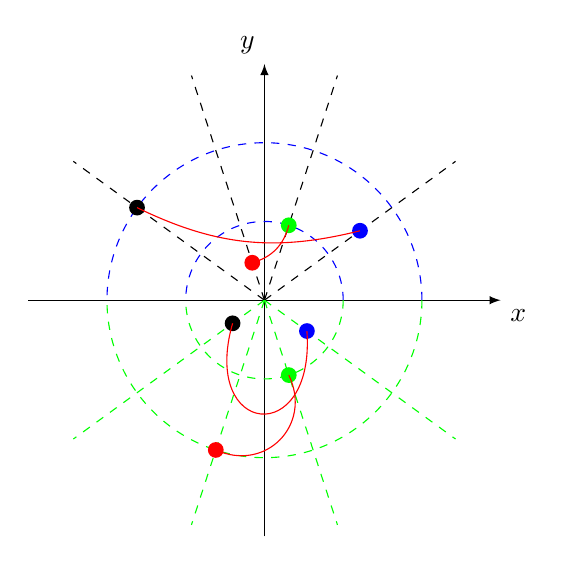
\begin{tikzpicture}
\draw[-latex] (-3,0) -- (3,0) node[pos=1,below right]{$x$};
\draw[-latex] (0,-3) -- (0,3) node[pos=1,above left]{$y$};

\draw[dashed] (0,0) -- (36:3);
\draw[dashed] (0,0) -- (72:3);
\draw[dashed] (0,0) -- (108:3);
\draw[dashed] (0,0) -- (144:3);

\draw[dashed, blue] (1,0) arc [start angle=0, end angle=180, radius = 1];
\draw[dashed, blue] (2,0) arc [start angle=0, end angle=180, radius = 2];

\coordinate (A) at (144:2);
\coordinate (B) at (108:1/2);
\coordinate (C) at (72:1);
\coordinate (D) at (36:1.5);

\fill[black] (A) circle [radius=0.1];
\fill[red] (B) circle [radius=0.1];
\fill[green] (C) circle [radius=0.1];
\fill[blue] (D) circle [radius=0.1];

\draw[red] (A) to [bend right=20pt] (D);
\draw[red] (B) to [bend right] (C);

\draw[dashed, green] (0,0) -- (-36:3);
\draw[dashed, green] (0,0) -- (-72:3);
\draw[dashed, green] (0,0) -- (-108:3);
\draw[dashed, green] (0,0) -- (-144:3);

\draw[dashed, green] (1,0) arc [start angle=0, end angle=-180, radius = 1];
\draw[dashed, green] (2,0) arc [start angle=0, end angle=-180, radius = 2];

\coordinate (IA) at (-144:0.5);
\coordinate (IB) at (-108:2);
\coordinate (IC) at (-72:1);
\coordinate (ID) at (-36:2/3);

\fill[black] (IA) circle [radius=0.1];
\fill[red] (IB) circle [radius=0.1];
\fill[green] (IC) circle [radius=0.1];
\fill[blue] (ID) circle [radius=0.1];

\draw[red] (IA) to [bend right=100, min distance=1.5cm] (ID);
\draw[red] (IB) to [bend right=70, min distance=0.7cm] (IC);
\end{tikzpicture}
\end{center}

\newpage

This is an inversion of an angle between two intersecting curves. Note that the curve from $p^\prime$ to $z^\prime$ is on the wrong side of the green secant line. For a non-draft, I would define a precise parametric curve or something.
\begin{center}
\begin{tikzpicture}[scale=3]
\draw[-latex] (-0.5,0) -- (2,0);
\draw[-latex] (0,-2) -- (0,2);

\draw[] (0,1) arc [start angle=90, end angle=-90, radius=1];

\draw[] (0,0) -- (30:2);
\draw[] (0,0) -- (-30:2);

\draw[dashed] (0,0) -- (15:2);
\draw[dashed] (0,0) -- (-15:2);

\fill[] (30:5/8) circle [radius=0.035] node[above]{$p$};
\fill[] (30:7/8) circle [radius=0.035] node[above left]{$q$};
\fill[] (15:6/8) circle [radius=0.035] node[below right]{$z$};

\draw[green] (15:6/8) -- (30:5/8);
\draw[green] (15:6/8) -- (30:7/8);

\draw plot [smooth] coordinates {(0:0.8)  (15:6/8)  (30:5/8) (60:0.5)}; 
\draw plot [smooth] coordinates {(0:0.6)  (15:6/8)  (30:7/8) (40:1.5)}; 

\fill[] (-30:1.6) circle [radius=0.035] node[below]{$p^\prime$};
\fill[] (-30:1.143) circle [radius=0.035] node[below]{$q^\prime$};
\fill[] (-15:4/3) circle [radius=0.035] node[below right]{$z^\prime$};

\draw[green] (-15:8/6) -- (-30:8/5);
\draw[green] (-15:8/6) -- (-30:8/7);

\draw[black] (-15:6/8) -- (-30:5/8);
\draw[black] (-15:6/8) -- (-30:7/8);

\draw[dotted] (30:5/8) -- (-30:5/8);
\draw[dotted] (30:7/8) -- (-30:7/8);
\draw[dotted] (15:6/8) -- (-15:6/8);

\draw plot [smooth] coordinates {(0:5/4)  (-15:8/6)  (-30:8/5) (-60:2)}; 
\draw plot [smooth] coordinates {(0:5/3)  (-15:8/6)  (-30:8/7) (-40:2/3)};

\coordinate (z) at (15:6/8);
\coordinate (p) at (30:5/8);
\coordinate (q) at (30:7/8);

\draw pic["$\alpha$",draw,-,angle eccentricity=1.4, angle radius=0.3cm]{angle=q--z--p};

\coordinate (iz) at (-15:8/6);
\coordinate (ip) at (-30:8/5);
\coordinate (iq) at (-30:8/7);

\draw pic["$\alpha$",draw,-,angle eccentricity=1.4, angle radius=0.3cm]{angle=iq--iz--ip};
\end{tikzpicture}
\end{center}

It is straight forward that
\[\angle pzq=\angle p^\prime z^\prime q^\prime\]
and this holds under the limit







\end{document}